\section{Evaluation}

% \begin{itemize}
%     \item Macro-benchmark
%         \begin{itemize}
%             \item BMC
%                 \begin{itemize}
%                     \item Expressiveness: how to evaluate?
%                         \begin{itemize}
%                             \item LOC: we have 33\% reduction
%                             \item 1 rust program vs 7 eBPF programs
%                             \item based on experience?
%                             \item Rust is a safer language
%                         \end{itemize}
%                     \item Performance evaluation
%                         \begin{itemize}
%                             \item Check their paper to see if we can perform
%                                 the same experiment
%                             \item We want a figure similar to Figure 6 in BMC
%                                 (except we don't need to evaluate on different
%                                 CPU configs)
%                             \item x: Vanilla memcached, BMC, Rust
%                             \item y: normalized throughput
%
%                         \end{itemize}
%                 \end{itemize}
%             \item Electrode
%                 \begin{itemize}
%                     \item LOC reduction
%                     \item Performance using their benchmark (similar to figure
%                         5 and 7 in Electrode)
%                     \item Dynamic allocation (ask the authors)
%                 \end{itemize}
%             \item LSM implementation (if we have time / requires handle
%                 nesting)
%             \item XRP
%             \item FUSE in eBPF (from Hubertus)
%         \end{itemize}
%     \item Micro-benchmark
%         \begin{itemize}
%             \item Memory footprint (BPF vs Rust) given we have a larger binary
%                 \begin{itemize}
%                     \item Number of prog in the same translation unit vs memory
%                         usage for program allocation
%                     \item This is because we are always statically linked to
%                         the runtime crate on the translation unit basis
%                     \item E.g. a bpf kern.c with 4 programs vs a rust main.rs
%                         with 4 programs
%                 \end{itemize}
%             \item Small expressiveness examples
%                 \begin{itemize}
%                     \item Loop: strcmp
%                     \item need more
%                 \end{itemize}
%             \item Stack-check overhead
%                 \begin{itemize}
%                     \item Use BMC?
%                     \item Or create some other workload that are function call
%                         intensive (since our instrumentation happens before
%                         each function call)
%                 \end{itemize}
%             \item Cleanup overhead on normal execution path (recording
%                 allocated kernel objects)
%                 \begin{itemize}
%                     \item Similar to Stack-check
%                 \end{itemize}
%             \item Startup overhead due to stack switching
%                 \begin{itemize}
%                     \item A minimal program () to show the upper bound?
%                     \item Plus a real world application (again BMC)?
%                 \end{itemize}
%         \end{itemize}
% \end{itemize}

\projname{} provides a new Linux extension framework that utilizes a safe
    programming language rather than the verifier.
In this section, we evaluate the usability as well as performance guided by the
    following questions:
\begin{enumerate}
    \item How does \projname{} provides better usability than eBPF and solve the
        verifier problems?
    \item Does the enhanced usability come at a cost of performance, especially
        for real world performance-sensitive programs?
    \item Are there other possible performance cost stemming from the design
        choices?
\end{enumerate}

\subsection{Usability evaluation}
The use of Rust in \projname{} eliminates the need to depend on a separate
    in-kernel verifier as in eBPF and therefore it is able to address the
    usability issues directly caused by the verifier.
At the same time, the rich builtin functionalty from a high-level language also
    allows developers to write simpler and cleaner code in real world use cases.
%We also take BMC~\cite{BMC} and implement it in \projname{} as a case study.

\subsubsection{Verifier issues from study}
We now revisit the verifier issues identified in our motivational study and
    demonstrate how \projname{} may solve them.

% \S~\ref{motivation:llvm-codegen} shows cases where fixes to codegen is needed
% root cause: real data field is hidden from user, and the field in user struct
%   is 32 bit -- the compiler/code-generator does not know about the real data
%   which is suppose to be a pointer.
% Therefore, the extra verification layer is to blame.
% With Rex there is no verification and everything (in this case, the data
%   layout) is known to the compiler.
% Talk a bit about how we handle this thing.
\para{LLVM codegen fix.} \S~\ref{motivation:llvm-codegen} demonstrates that
    user intervention is needed to fix problems where sometimes the code generated
    by the compiler is not taken by the verifier.
The core of the problem, is the extra verification layer of eBPF, which creates
    a gap between the developer/compiler and the verifier.
The field being accessed is only visible to the compiler as a 32-bit integer,
    rather than its underlying 64-bit pointer type hiden by the verification
    step (\S~\ref{motivation:llvm-codegen}).

This problem will not manifest in \projname{}.
This is because \projname{} implements information hidding without the use of
    the extra verification layer.
Instead, \projname{} utilizes private fields of Rust structs to hide the unused
    information and the kernel crate exposes the useful fields with the type
    they are supposed to be used in extension programs.
For example, the \texttt{data} field is exported to extension programs as a
    character data slice, since it points to the data content of a packet.
In this way, all operations associated with these fields are visible to the
    compiler, which in turn could generate correct code.

\para{Program restructuring for verifier}
Our study reveals that many of times the instruction limit on the verifier
    forces developers to either split their program into multiple small pieces
    or refactor their code to eliminate extra instructions that the verifier
    may have to go through.
One of the representative example of these cases is the BMC project~\cite{BMC},
    where the authors have to not only write seven small programs but also
    bound the data size through the use of cumbersome loop conditions.
eBPF programs may have to be refactored for expressiveness reasons as well,
    as the verifier limits what eBPF programs can do.
None of these problems would appear in \projname{}, which does not
    have a verifier and does not limit the size of extension programs.

% We demonstrate the benefit of \projname{} through our case study on BMC
%     (\S~\ref{eval:bmc-case-study}).

\para{Add specific code to pass verifier.}
\S~\ref{motivation:add-code} demonstrates cases where the verifier loses track
    of certain verification states and therefore forces developers to
    choose a specific implementation, even though other rejected
    implementations are totally safe and sound.

For \projname{}, the Rust compiler may reject a program if the program does not
    fit in what it deems as safe (e.g. writing to a static variable is deemed
    unsafe even if the program will only be executed in a single threaded
    mode).
However, the use of Rust in \projname{} eliminates the extra verification layer,
    which in turn removes the gap between the developer and the verifier.
The programmer only needs to keep the mental model of Rust instead of having a
    separate and different one for the verifier.
The Rust compiler can also provide hints about what went wrong that are much
    easier to understand and use than verifier logs.

\jinghao{As I said, I think the Rust compiler may also reject some code that
    are actually safe. So it seems that we also have the same problem. Therefore
    I'm trying to make an argument on that we do not have the gap.}

\para{Implement kernel-version-specific fixes.}
Some of the verification issues in eBPF are due unfixed verifier bugs in
    previous kernel versions, as shown in \S~\ref{motivation:kernel-version},
    where the developers have to address the bug by changing their
    implementation.
The same problem also presents in \projname{}, because the Rust compiler is not
    free of bugs.
Programmers will have to address the unfixed compiler bugs in older versions
    in case they hit the problem.

On the other hand, the version of Rust used is decoupled from the kernel version, while
    with eBPF the verifier version is tied to the kernel version.
This would allow developers to potentially use a more recent Rust compiler version with
    bug fixes on older kernels instead of porting fixes to previous versions.
\milo{Is there some benefit here due to having Rust compiler version decoupled from kernel version?}

\para{Add Pruning Checkpoints.}
Because the verifier has an upper limit on the number of instructions it can
    process, some eBPF projects use ``pruning checkpoints'' to reduce
    verification complexities for programs (\S~\ref{motivation:checkpoint}).
This will not be a problem of \projname{}, because switching to Rust means that
    programs now can have arbitrary length, and the compiler can still process
    them.

\subsubsection{Case study: \projname{}-BMC}
\label{eval:bmc-case-study}

\begin{figure}[t]
    \lstinputlisting[language=Rust]{./snippets/s6-rust.rs}
    \vspace{-10pt}
    \caption{Packet parsing code for cache invalidation in \projname{}}
    \vspace{-10pt}
    \label{fig:rust-code}
\end{figure}

% \jinghao{Add some sentence saying this is a prevalent pattern in BMC?}
% \jinghao{Can we make the claim that this complexity is for passing the
%     verifier?}
% During implementation of function \texttt{bmc\_invalidate\_cache},
%     we assume that each pcket

% This discovery highlighted the obscurity and susceptibility to errors inherent
%     in the original code structure, primarily due to the complex judgment
%     conditions buried within nested if statements.

% Rex-BMC
% 1. eliminates verifier-related checks
% 2. simplifies the code bc of Rust core library

We re-implement BMC\cite{BMC} in \projname{} (\projname{}-BMC) to demonstrate the
    enhanced usability.
The resulting program is not a direct translation from the original eBPF
    version in C, rather, we implement the same high-level logic but with
    slight deviations from BMC where the enhanced usability and expressiveness
    of Rust allows a simpler implementation.

% \projname{}-BMC is able to avoid the complexities caused by the verifier.
In \projname{}-BMC, the builtin language features and libraries of Rust not
    only allows the revmoval of verifier-specific checks but also faciliates
    cleaner and simpler code.
The equivalent cache invalidation code in \projname{} to
    \S~\ref{motivation:restructure} is shown in Figure~\ref{fig:rust-code}.
The checks required previously by the verifier, including these for offset and
    \texttt{data\_end} limits, are now being enforced via the inherent language
    features of Rust, such as the \texttt{slice} that implements bound checks
    (L2 and L10).
The check on \texttt{BMC\_MAX\_PACKET\_LENGTH}, serving as a constraint to minimize the number
    of jump instructions to circumvent the eBPF verifier, is no longer necessary
    in the Rust code.
At the same time, specific checks such as the ones for identified SET commands
    and the \texttt{key\_found} state can implemented with built-in
    functions and closures in an easy and clean way (L4-L6 and L11).
% \jinghao{ We should also talk about \texttt{BMC\_MAX\_PACKET\_LENGTH}.}
% Meanwhile, other checks, including those for offset and \texttt{data\_end} limits, are being enforced via
%     the inherent language features of Rust, such as the \texttt{slice} that implements bound checks.

% \jinghao{Need a few sentences to explain why a bunch of checks are no
%     longer needed and why we are safe even without these checks.}
% \jinghao{The four levels of nesting in the original code is significantly...}
% \juowen{break as two paragraphs}

% For the loops in the original implementation, \projname{}-BMC utilizes the
%     lazily evaluated \texttt{windows}, \texttt{enumerate} and
%     \texttt{filter\_map} from slice iterators.
% % Refer back to BMC code, the similar logic is implemented in \projname{}-BMC as shown in Figure~\ref{fig:rust-code}.
% These methods split the whole payload into chunks
%     of 4 bytes, and collects the results for which the chunk equals the keyword
%     of SET commands into iterators.
% % \jinghao{What are these challenges -- are we still in the context of cache
% %     invalidation? By the way, can we abstract this out to all ``loops'' in BMC?
% % At the same time, we probably need to explain what \texttt{filter\_map} does.}
% % This approach facilitates the creation of an iterator, which is instrumental in identifying
% %     the quantity of SET commands present in the current packet payload.
% With the creation of the iterators, the number of SET commands present in the
%     current packet payload can be easily identified.
% Further enhancing the ease of programming and the readability, Rust's syntactic sugar is employed for
%     iterating over the identified memcached SET commands, streamlining the process.
% % \jinghao{The four levels of nesting in the original code is significantly...}
% The four levels of nesting in the original code is significantly reduced by
% converting a \texttt{for}-loop with intricate conditions into a clean chain
%     of higher-order functions with closures.
% % \jinghao{lambda function -> a clean chain of higher-order functions with
% %     lambda function?}
% This conversion is achieved through the utilization of \texttt{take\_while}.
%     With the iterator from \texttt{filter\_map}, \texttt{take\_while} will
%     filter the memcached SET key from the payload, thus dividing the code into three distinct
%     sequential parts and markedly improving its expressiveness.

% \juowen{ How to connect what we mentioned before ralated to limit of verifier? }
% \jinghao{I think the current writing is good, just need some more polishing}

% In the \projname{}-BMC, constraints associated with the verifier are nonexistento.
At the same time, due to the absence of the program size limit in \projname{}-BMC,
% Therefore, program doesn't have to put the metadata in a seperated map,
%     which significantly obscure the logic of program and may undermine the performance.
    developers no longer have to put the computation state in a seperated map
    in order for them to be persistent across tail calls, which leads
    to clearer and potentially more efficient programs.

% \jinghao{@Ruowen pls take a look.}
% \juowen{It feels weird leaving this thing here, feels like not convincing}

% \jinghao{Can we also write maybe one paragraph on the need to store the parsing
%     context across tail calls?}
% \jinghao{Also should explain what \texttt{take\_while} does.}
% \jinghao{Now it feels like we should make part larger, i.e., include code
%     examples and show how Rust helps with that.
% We can then move this part into the new qualitative evaluation.}

\subsection{Macrobenchmark evaluation}
\label{eval:macro}
We now demonstrate that enhanced usability of \projname{} does not come at a
    cost of performance.
Through our \projname{}-BMC implementation, we show that \projname{} can handle
    such complicated and performance-sensitive use cases from the real world.
Overall, \projname{}-BMC is able achieve a throughput of 1.111M requests per
    second when running on 8 cores -- comparable to that of eBPF-BMC (1.106M).

% \subsubsection{\projname{}-based BMC}
% \jinghao{TODO: Preamable}
% BMC implements in-kernel memcached cache -- how it works
% Compilcated program, original paper splits into 7 programs and uses tail calls
%

%\para{Experiment setup}
Our evaluation setup consists two machines, with one
    acting as the server and the other one acting as the client.
The server machine runs the \projname{} custom kernel based on Linux v5.15.0 on
    an AMD EPYC 7551P 32-Core processor with 112 GB memory.
SMT and Turbo are turned off for the experiments.
The client machine runs a vanilla v6.8.0 Linux kernel on AMD Ryzen 9 7900X
    processor with 128 GB memory.
Both machines are equiped with Mellanox ConnectX-3 Pro 40GbE NICs and are
    connected back-to-back using a single port.

% Key: 16 bytes, value: 32 bytes
% 50 million with Zipf 0.99
% 10 GB memcached, 2.5 GB BMC
% Preload all keys
% GET:SET 30:1

We use the following workload to evaluate our \projname{}-BMC together with the
    original eBPF-BMC.
Our dictionary contains 50 million Memcached keys following a Zipf
    distribution with 0.99 skewness.
All keys are 16 bytes in size and are paired with 32-byte values in the
    experiments.
The storage sizes of the Memcached and BMC are set to 10 GB andBMC 2.5 GB,
    respectively.
According to the calculation in the original work, all items
    can be stored in Memcached itself but only 6.3 million of them can fit in
    BMC.
Before experiments, the Memcached server is pre-loaded with all keys by
    sending TCP SET requests for each key in the dictionary from the client.
The client then sends requests to the server with a 30:1 ratio betweren UDP GET and
    TCP SET requests and measures the throughput.

We evaluate the throughput of three setups: MemcachedSR (from BMC),
    MemcachedSR+BMC, and MemcachedSR+\projname{}-BMC.
The original open-sourced BMC code targets Linux kernel version 5.3.0 and we
    port it to the v5.15.0 \projname{} kernel for the evaluation.
For each setup, we vary the number of processor cores and the number of threads
    used by the Memcached server and pin each thread onto each core.
We also adjust the CPU affinity of IRQs associated with the NIC such that the
    network interrupts are processed on the same set of cores the Memcached
    server executes on.

\begin{figure}[t]
    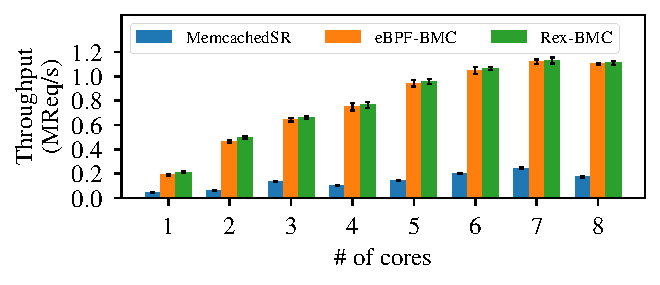
\includegraphics[width=1.0\linewidth]{figs/bmc.pdf}
    \centering
    \vspace{-25pt}
    \caption{Throughput of MemcachedSR, eBPF-BMC, and \projname{}-BMC
        under different number of CPUs/threads.
    }
    \label{fig:eval-bmc}
    \vspace{-12pt}
\end{figure}

Figure~\ref{fig:eval-bmc} shows the throughput of the three setups under
    different numbers of CPUs and threads.
MemcachedSR processes all requires in userspace and thus its throughput suffers
    from the overhead of the kernel network stack, achieving only 45K requests
    per second under a single thread and 175K requests per second under 8
    cores.
On the other hand, both eBPF-based and \projname{}-based BMC are able to
    achieve a much higher throughput because they can process a large
    fraction of requests at NIC driver level and without the need of going through
    the expensive kernel network stack.
With 8 CPU cores and threads, eBPF-BMC and \projname{}-BMC achieve a thoughput
    of 1.106M and 1.111M, and a performance benefit of 6.3x and 6.4x,
    respectively.
It is also clear that \projname{} is able achieve a better usability while
    keeping the same level of performance and safety guarrantee comparing to
    eBPF,  as the throughput of \projname{}-BMC is comparable to that of
    eBPF-BMC under all CPU/thread setups.

\subsection{Microbenchmark evaluation}
Our design choices of \projname{} could introduce additional performance
    overheads on.
In this section, we implement microbenchmark cases for the potential
    performance overheads and demonstrate that although overheads may be
    present in pessimistic cases, they have neglegible impact in real world use
    cases.
All experiments are performed on the same machine that acts as the server in
    \projname{}-BMC experiments (\S~\ref{eval:macro}).

\subsubsection{Static memory footprint}
\label{eval:mem-footprint}
\begin{figure}[t]
    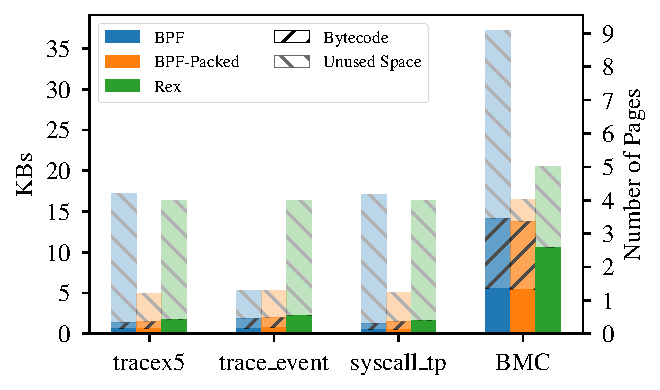
\includegraphics[width=1.0\linewidth]{figs/mem.pdf}
    \centering
    \vspace{-25pt}
    \caption{Amount of pages allocated and actual memory occupied by various
        eBPF and \projname{} programs}
    \label{fig:eval-mem-footprint}
    \vspace{-10pt}
\end{figure}
% definition of memory footprint
% eBPF only have JIT code
% Rust have code sections and other sections, e.g. data and GOT sections
We evaluate how the in-kernel memory footprint of \projname{} programs
    compares to that of eBPF programs.
We found that \projname{} incurs fair amount of overhead on memory footprint
    when there are only few programs defined and compiled together, due to how
    program code and data are organized in the executable.
However, with more programs compiled in the same executable, the overhead
    becomes amortized and the overall memory footprint becomes more efficient.

We define the memory footprint as the number of static memory pages required
    for program execution.
For eBPF, this only includes the post-JIT native code, since eBPF program does
    not support static data sections.
% For \projname{} this includes all load segments from the compiled ELF
%     executable, which consists not only the text sections, but also the data
%     sections for static variables (e.g., program objects and maps objects) as
%     well as the sections that implement support for position-independent code
%     (e.g., GOT sections).
For \projname{}, this includes all \texttt{LOAD} segments from the compiled ELF
    executable.
A compiled \projname{} program generally has four \texttt{LOAD} segments that
    map to relocations, text, read-only data, and the GOT.
%     map to different sections (e.g. text, rodata, etc).

In this experiment, we compare the memory required for both
    \projname{} programs and their equivalent eBPF programs.
We select 3 simple eBPF programs from the sample eBPF programs shipped with the
    kernel -- the trace point program \texttt{syscall\_tp}, the kprobe program
    \texttt{tracex5} and the perf event program \texttt{trace\_event}.
We also include the BMC program (\S~\ref{eval:bmc-case-study}) in the
    experiment because it represents an example of a more complicated use case.
We implement a \projname{} version for each of the programs.

The number of pages allocated for and the actual amount of memory used by the
    eBPF programs and their \projname{} counterparts are shown in
    Figure~\ref{fig:eval-mem-footprint}.
% In general, the memory footprint becomes more efficient for \projname{} when
%     more programs are defined in the same source file. \jinghao{or should we
%     say ``project''}
Before Linux 5.18, each eBPF program occupied dedicated pages.
eBPF then introduced the ``packed allocation''
    feature~\cite{bpf-packed-alloc}, which
    tries to pack different programs into the same page to use memory more
    efficiently.
% and is labeled in Figure~\ref{fig:eval-mem-footprint} as
%     ``BPF-Packed''.
For \projname{}, multiple programs in the same project are
    loaded together in the same executable.
However, different segments of the executable have to reside in their own
    pages since they require different memory permissions.

Because each segment of a \projname{} program needs its own page, \projname{}
    exhibits a higher static memory footprint for all programs when compared to
    eBPF with packed allocation.
When comparing to eBPF without packed allocation, \projname{} is more efficient
    when more programs are defined in the same project.
\texttt{trace\_event} represents a case where only a single extension program
    is defined.
For such cases, \projname{} would exhibit a larger memory footprint, because of
    its extra segments in addition to code.
%     its executable contains other sections (e.g., data and relocations) in
%     addition to code.
For \texttt{tracex5} and \texttt{syscall\_tp}, eBPF and \projname{} uses the
    same number of memory pages
    since both of them consist of 4 programs, and one page per program is
    allocated without packed allocation.
For BMC, \projname{} achieves a more efficient memory footprint.
The original eBPF-BMC has to be split into 7 programs in order to keep it
    within the limit of the verifier.
Doing so without packed allocation makes each program occupy its own pages.
The \projname{}-BMC has all the code packed in the text section, and therefore
    utilizes the memory more efficiently.

% \jinghao{TODO: Might want to discuss the larger ocupied memory in \projname{} than eBPF}

% \begin{itemize}
%     \item need a figure: bar graph showing the memory footprint of bpf and
%         \projname{} programs on our sample programs
%     \item sample programs: \texttt{syscall\_tp}, \texttt{tracex5},
%         \texttt{trace\_event}, and BMC.
%     \item y: total number of pages allocated for the loaded object (JIT-ed code
%         for BPF, loaded and mapped pages for Rust)
% \end{itemize}

\subsubsection{Startup overhead due to stack switching}
\begin{table}[t]
    \small
    \centering
    \begin{tabular}{ccc}%{|p{6cm}|p{1cm}|}
        \toprule
        \textbf{Extension} & \textbf{Empty prog runtime} & \textbf{Spinlock runtime} \\
        \midrule
        eBPF & 43.5 $\pm$ 4.79 ns & 256.8 $\pm$ 142.4 ns\\
        \projname{} & 44.1 $\pm$ 4.93 ns & 254.5 $\pm$ 192.3 ns\\
        \bottomrule
    \end{tabular}
    \caption{Empty program runtime as well as spinlock acquire and release
        runtime for eBPF and \projname{} in nanoseconds}
    \vspace{-25pt}
    \label{tab:startup-cleanup}
\end{table}

We then show that the support for a dedicated program stack in \projname{} does
    not incur performance overhead on program startup and exit, with the
    runtime of an empty \projname{} staying within 1ns the runtime of an empty
    eBPF program.

\projname{}'s usage of a dedicated stack for execution and the implementation
    of exception handling support may incur additional overhead during program
    startup and shutdown.
This design requires saving of the stack and frame pointer and replacing them
    with the top address of the dedicated stack before starting the program,
    and restoring the saved stack and frame pointer after the program exits.
The manipulation of the stack pointers adds to six more memory instructions to
    the dispatcher function of the \projname{} programs.
In this experiment we measure the overhead of these stack pointer operations.
We implement an empty kprobe extension program -- both in eBPF and in
    \projname{} -- and measure their wall runtime including the program
    dispatcher function.
The result is shown in Table~\ref{tab:startup-cleanup}.
On average, the difference of runtime of invoking an empty \projname{} and eBPF
    program is less than 1ns.
This shows the additional stack pointer manipulations needed by \projname{}
    contributes negligible overhead.

\subsubsection{Helper function overhead}
\label{eval:inline}

% The raw data and script used to make the graph (plot2.py)
% is in the map-test directory under testing/analysis/impl:ctx-converison
\begin{figure}[t]
    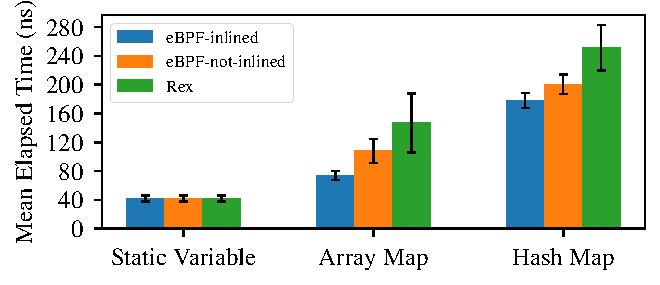
\includegraphics[width=1.0\linewidth]{figs/inline.pdf}
    \centering
    \vspace{-25pt}
    \caption{Runtime of map lookups on various setups}
    \label{fig:eval-inline}
    \vspace{-12pt}
\end{figure}

% \begin{itemize}
%     \item inline v.s. out-of-line map helpers
%         \begin{itemize}
%             \item table showing runtime of a map lookup operation in a eBPF and
%                 a Rust program
%             \item the kernel will automatically inline lookup in BPF
%             \item Rust version will not get inlined
%             \item measurement can be in ns for now, but better if it could be
%                 in cycles
%             \item maps to test: array, hash (htab-lru, xsk-map?)
%         \end{itemize}
% \end{itemize}
We evaluate the impact of missed opportunities due to the elimination of
    the eBPF verifier in \projname{} by looking into the eBPF map lookup
    helpers.
%  Specifically, we look into the optimization of eBPF map lookups.
The map lookup helpers represent a pessimistic case for \projname{} because
    \projname{} not only misses the load time optimization but also needs more
    wrapping code than other helpers due to its map implementation.
We found that the missed optimization slows down the helper call by around 30ns
    and the safe wrapping code adds another 45ns, which is acceptable for a
    pessimistic case.

The eBPF verifier can inline the \texttt{bpf\_map\_lookup\_elem}
    helper function by replacing the call into equivalent eBPF instructions.
This optimization can avoid two function calls and two pointer dereferences for
    map types that support lookup inlining.
However, in \projname{}, inlining is not performed due to the absence of the
    eBPF verifier as well as kernel internal information (e.g. map addresses).

We measure the runtime of eBPF map lookups under three
    settings, eBPF with inlining, eBPF without inlining, and \projname{}.
Our test program for both eBPF and \projname{} is a tracepoint program that
    uses the \texttt{bpf\_ktime\_get\_ns} helper to measure the runtime of
    a \texttt{bpf\_map\_lookup\_elem} call.
The \texttt{bpf\_map\_lookup\_elem} invocation is by defualt inlined by the
    eBPF verifier when possible.
The setup of eBPF without inlining is achieved by removing the inlining logic
    from the eBPF verifier.
We selected two commonly-used eBPF map types for this experiment: array maps
    and hash maps.
Both of them support lookup inlining.

% Figure~\ref{fig:eval-inline}
% shows the performance of inlining and non-inlining on a vanilla
% v5.15 kernel as well as the \projname{} implementation.
Figure~\ref{fig:eval-inline} shows the performance of map lookups under the
    three different setups on different maps.
% The vanilla non-inlined
% kernel is achieved by commenting out the lines in the kernel verifier.c file that
% automatically inlines the bpf\_map\_lookup\_elem method.
For both array maps and hash maps, the
    runtime of map lookup can be reduced by 20-30 ns compared to eBPF without
    inlining.
% In the graph,
% the performance impact of inlining the method is 20-30 nanoseconds.
% The additional slowdown of 30-40 nanoseconds seen in the rust implementation
% can be explained by the wrapping performed around the bpf\_map\_lookup\_elem method.
An additional slowdown of 30-40 nanoseconds is present for map lookups in
    \projname{}.
This is because of the wrapping code around the kernel
    \texttt{bpf\_map\_lookup\_elem} that allows \projname{} programs to invoke
    it using safe Rust objects.
For most of other helper functions, neither do they support such load time
    optimizations in eBPF nor do they require the amount of wrapping code as in
    map helpers, therefore, they would have a performance similar to that of
    eBPF's.

\jinghao{TODO: Rust atomics discussions, possibly with something from the nomicon}

% Egor: Not sure if I should go into more technical details about whats going on
% in the wrapping

% Using libbpf (and libiu in the case of \projname{}) the sample \projname{} or c bpf
% program is loaded and attached to a tracepoint which is then called by the trigger.
% In the instance of the inlined and non-inlined tests this tracepoint is getcwd, and
% in the instance of the rust tests that tracepoint used is sys\_enter\_dup. The
% triggers consist of a one-line c program that calls the appropriate function such as getcwd().
% The bpf program creates the corresponding map and measures the time
% it takes to execute a single map\_lookup\_elem. This time is measured with
% bpf\_ktime\_get\_ns() and then printed with bpf\_printk() and recorded.
% \milo{Maybe we should talk about why we chose these specific maps. i.e. that array and hash maps are the main ones that support the inlining?}

\subsubsection{Runtime cost of safety in \projname{}}
The cleanup mechanism for exception handling and runtime stack instrumentation
    could incur additional performance overheads.
Here, we evaluate the performance impact from these runtime instrumentations.
Our result shows that the cleanup mechanism on non-exceptional execution adds
    no observable overhead, and that recursions in \projname{} with runtime
    stack instrumentation can execute more efficiently than the same logic
    implemented in eBPF using tail calls.

\para{Cleanup overhead on normal execution path}
% \begin{table}[t]
%     \small
%     \centering
%     \begin{tabular}{cc}%{|p{6cm}|p{1cm}|}
%         \toprule
%         \textbf{Extension} & \textbf{Runtime of acquiring \& release a lock (ns)} \\
%         \midrule
%         eBPF & 256.8 $\pm$ 142.4 \\
%         \projname{} & 254.5 $\pm$ 192.3 \\
%         \bottomrule
%     \end{tabular}
%     \caption{Runtime of spinlock acquire and release for eBPF and \projname{}}
%     \vspace{-10pt}
%     \label{tab:cleanup-overhead}
% \end{table}
The safe cleanup mechanism employed by \projname{} requires recording the allocated
    resource at runtime, which, compared to eBPF or Itanium C++ ABI, adds extra
    runtime overhead.
We therefore evaluate the runtime overhead from \projname{}'s cleanup
    mechanism.
For this miscrobenchmark, we choose to use a program that acquires and then
    immediately releases a BPF spinlock.
Since the acquired spinlock is a resource that needs to be released upon Rust
    panics, \projname{}'s cleanup mechanism needs to record it in its per-CPU
    buffer.
The program is implemented both in eBPF and \projname{} and the time used to
    acquire and release the spinlocks are measured.
As shown in Table~\ref{tab:startup-cleanup}, the runtime difference between
    eBPF and \projname{} is less than 2ns with \projname{} being the faster
    one, implying the overhead of \projname{}'s cleanup mechanism is
    negligible.

\para{Stack-check overhead}
\begin{figure}[t]
    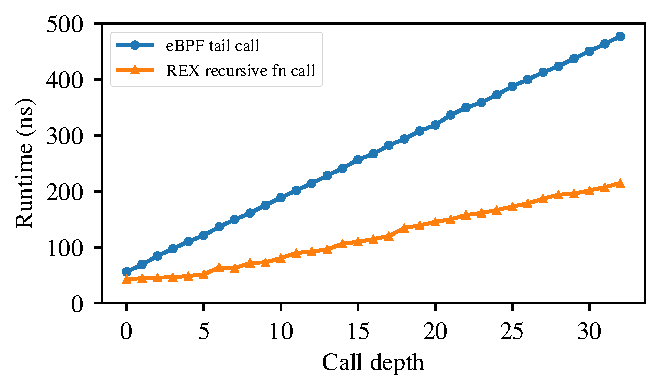
\includegraphics[width=1.0\linewidth]{figs/recursive.pdf}
    \centering
    \vspace{-25pt}
    \caption{Runtime of eBPF tail calls and \projname{} recursive calls with
    stack instrumentation}
    \label{fig:eval-recursion}
    \vspace{-10pt}
\end{figure}
% We then evaluate how much overhead the runtime stack check have on the
%     performance of \projname{} programs.
The stack instrumentation is added before each
    function call in the \projname{} program if the program contains indirect
    or recursive function calls that prevents the compiler from calculating the
    stack usage statically.
In this experiment, we implement a recursive program in both
    eBPF and \projname{}.
The recursive function calls itself for a specifed number of times and contains
    no other code.
Since eBPF does not natively support recursive functions, we use eBPF tail
    calls to implement the same logic.
In \projname{}, we use the \texttt{black\_box} hint from the Rust core library
    to prevent the compiler from optimizing away the recursive call.
Figure~\ref{fig:eval-recursion} plots the runtime of the recursive code against
    the depth of the call stack from 0 to 32.
The kernel imposes a hard limit of 32 on the number of tail calls an eBPF
    program can perform.
Even with the stack check instrumentation in place, \projname{} is able to
    achieve roughly half the runtime of eBPF.
This is likely because of the overhead of runtime checking on whether the tail
    call limit has been reached and verification of tail call targets in eBPF.
